\documentclass[10pt,winfonts,fancyhdr,hyperref,UTF8]{ctexrep}
\usepackage{indentfirst} 
\usepackage{fontspec}
\usepackage{titlesec}
\usepackage{xeCJK}
\usepackage{graphicx}
\usepackage{ifthen}
\usepackage{color,fancyvrb}
\usepackage{listings}
\usepackage{syntonly}
\usepackage{makeidx}
\usepackage[hidelinks, colorlinks=true]{hyperref}
\usepackage{algorithm}
\usepackage{algpseudocode}
\usepackage{amssymb}
\usepackage{multirow}
\usepackage{ulem}
\usepackage{diagbox}
\makeatletter
%LeetCode Setting
\usepackage[centering,paperwidth=180mm,paperheight=230mm,%
body={390pt,530pt},marginparsep=10pt,marginpar=50pt]{geometry}
\usepackage{color}
\usepackage{enumitem}
\usepackage{fancyvrb}
\usepackage[bottom,perpage,symbol*]{footmisc}
\usepackage{graphicx}
\usepackage[hidelinks]{hyperref}
\usepackage{makeidx}
\usepackage[toc]{multitoc}
\usepackage{pifont}
\usepackage{underscore}
\usepackage{amsmath}

\DefineFNsymbols*{chinese}{{\ding{172}}{\ding{173}}{\ding{174}}{\ding{175}}%
{\ding{176}}{\ding{177}}{\ding{178}}{\ding{179}}{\ding{180}}{\ding{181}}}
\setfnsymbol{chinese}

\hypersetup{bookmarksnumbered=true,bookmarksdepth=2}

\CTEXsetup[number={\thechapter}]{chapter}
\CTEXsetup[format+={\raggedleft}]{chapter}
\CTEXsetup[beforeskip={10pt}]{chapter}
\CTEXsetup[afterskip={30pt}]{chapter}
\def\CTEX@chapter@aftername{\par} % \CTEXsetup[aftername={\par}]{chapter}
\CTEXsetup[format+={\raggedright}]{section}
\CTEXsetup[beforeskip={-3.0ex plus -1ex minus -.2ex}]{section}
\CTEXsetup[afterskip={2.3ex plus .2ex minus 0.2ex}]{section}

\renewcommand \thefigure{\thechapter-\arabic{figure}}
\renewcommand \thetable{\thechapter-\arabic{table}}

\newcommand\figcaption[1]{\def\@captype{figure}\caption{#1}}
\newcommand\tabcaption[1]{\def\@captype{table}\caption{#1}}

\long\def\@caption#1[#2]#3{%
  \addcontentsline{\csname ext@#1\endcsname}{#1}%
    {\protect\numberline{\csname fnum@#1\endcsname}{ \ignorespaces #2}}% change "the" to "fnum@"
    \normalsize
    \@makecaption{\csname fnum@#1\endcsname}{\ignorespaces #3}}

\long\def\@makecaption#1#2{%
  \vskip\abovecaptionskip
  \sbox\@tempboxa{#1\quad#2}%
  \ifdim \wd\@tempboxa >\hsize
    #1\quad#2\par
  \else
    \global \@minipagefalse
    \hb@xt@\hsize{\hfil\box\@tempboxa\hfil}%
  \fi
  \vskip\belowcaptionskip}

\setlength\abovecaptionskip{0pt}
  
\setmainfont{Times New Roman}
%\setmainfont{Linux Libertine}
%\setmainfont{TeX Gyre Pagella}
\newfontfamily\urlfont{Times New Roman}
%\setmonofont[AutoFakeBold=1.6,AutoFakeSlant=0.17,Mapping=tex-text-tt]{Inconsolata}
\setCJKfamilyfont{zhyou}{YouYuan}

\newcommand{\fn}[1]{\texttt{#1}}
\newcommand{\sfn}[1]{\texttt{\small #1}}
\newcommand{\kw}[1]{\textsf{#1}}
\newcommand{\myurl}[1]{{\urlfont #1}}
\newcommand{\mpar}[1]{\marginpar[\hfill\kaishu #1]{\kaishu #1}}
\newcommand{\mn}[1]{\texttt{\bs #1}}
\renewcommand{\today}{\the\year-\the\month-\the\day}
\newcommand\bs{\textbackslash}
\newcommand{\code}[1]{\small{\fontspec{Latin Modern Mono} #1}}

\newcommand\begindot{\begin{itemize}
[itemsep=2pt plus 2pt minus 2pt,%
topsep=3pt plus 2pt minus 2pt,%
parsep=0pt plus 2pt minus 2pt]}
\newcommand\myenddot{\end{itemize}}

\newcommand\beginnum{\begin{enumerate}
[itemsep=2pt plus 2pt minus 2pt,%
topsep=3pt plus 2pt minus 2pt,%
parsep=0pt plus 2pt minus 2pt]}
\newcommand\myendnum{\end{enumerate}}

\DefineVerbatimEnvironment%
  {Code}{Verbatim}
  {fontsize=\small,baselinestretch=0.9,xleftmargin=3mm}

\raggedbottom
%\setlength{\parskip}{1ex plus .5ex minus .5ex}

\def\FV@SetLineWidth{%
  \if@FV@ResetMargins\else
    \advance\leftmargin\@totalleftmargin
  \fi
  \advance\leftmargin\FV@XLeftMargin\relax
  \advance\rightmargin\FV@XRightMargin\relax
  \linewidth\hsize
  %\advance\linewidth-\leftmargin
  %\advance\linewidth-\rightmargin
  \hfuzz\FancyVerbHFuzz\relax}


\def\FV@SingleFrameLine#1{%
%% DG/SR modification end
  \hbox to\z@{%
    %\kern\leftmargin
%% DG/SR modification begin - Jun. 22, 1998
    \ifnum#1=\z@
      \let\FV@Label\FV@LabelBegin
    \else
      \let\FV@Label\FV@LabelEnd
    \fi
    \ifx\FV@Label\relax
%% DG/SR modification end
      \FancyVerbRuleColor{\vrule \@width\linewidth \@height\FV@FrameRule}%
%% DG/SR modification begin - Jun. 22, 1998
    \else
      \ifnum#1=\z@
        \setbox\z@\hbox{\strut\enspace\urlfont\FV@LabelBegin\strut}%
      \else
        \setbox\z@\hbox{\strut\enspace\urlfont\FV@LabelEnd\strut}%
      \fi
      \@tempdimb=\dp\z@
      \advance\@tempdimb -.5\ht\z@
      \@tempdimc=\linewidth
      \advance\@tempdimc -\wd\z@
      %\divide\@tempdimc\tw@
      \ifnum#1=\z@              % Top line
        \ifx\FV@LabelPositionTopLine\relax
          \FancyVerbRuleColor{\vrule \@width\linewidth \@height\FV@FrameRule}%
        \else
          \FV@FrameLineWithLabel
        \fi
      \else                     % Bottom line
        \ifx\FV@LabelPositionBottomLine\relax
          \FancyVerbRuleColor{\vrule \@width\linewidth \@height\FV@FrameRule}%
        \else
          \FV@FrameLineWithLabel
        \fi
      \fi
    \fi
%% DG/SR modification end
    \hss}}


%% DG/SR modification begin - May. 19, 1998
\def\FV@FrameLineWithLabel{%
  \ht\z@\@tempdimb\dp\z@\@tempdimb%
  \FancyVerbRuleColor{%
    \raise 0.5ex\hbox{\vrule \@width\@tempdimc \@height\FV@FrameRule}%
    \raise\@tempdimb\box\z@}}
%% DG/SR modification end


\def\FV@EndListFrame@Lines{%
  \begingroup
    %\vskip 0.5ex
    \baselineskip\z@skip
    \kern\FV@FrameSep\relax
%% DG/SR modification begin - May. 19, 1998
%%    \FV@SingleFrameLine
    \FV@SingleFrameLine{\@ne}%
%% DG/SR modification end
  \endgroup}

\newskip\mytopsep
\setlength{\mytopsep}{4pt plus 2pt minus 3pt}

\def\FV@ListVSpace{%
  \@topsepadd\mytopsep
  \if@noparlist\advance\@topsepadd\partopsep\fi
  \if@inlabel
    \vskip\parskip
  \else
    \if@nobreak
      \vskip\parskip
      \clubpenalty\@M
    \else
      \addpenalty\@beginparpenalty
      \@topsep\@topsepadd
      \advance\@topsep\parskip
      \addvspace\@topsep
    \fi
  \fi
  %\showthe \@topsepadd
  %\showthe \topsep
  %\showthe \partopsep
  %\showthe \parskip
  \global\@nobreakfalse
  \global\@inlabelfalse
  \global\@minipagefalse
  \global\@newlistfalse}

\def\FV@EndList{%
  \FV@ListProcessLastLine
  \FV@EndListFrame
  %\showthe \@topsepadd
  \@endparenv
  \endgroup
  \@endpetrue}

\def\theFancyVerbLine{\sffamily\scriptsize\arabic{FancyVerbLine}}

\DefineVerbatimEnvironment%
  {Codex}{Verbatim}
  {fontsize=\small,baselinestretch=0.9,xleftmargin=3mm,%
  frame=lines,labelposition=all,framesep=5pt}

\DefineVerbatimEnvironment%
  {Code}{Verbatim}
  {fontsize=\small,baselinestretch=0.9,xleftmargin=3mm}

\makeindex

%Other settings:
\lstset{%  
  alsolanguage=Java,  
  language={C++},
  tabsize=4, %  
  frame=shadowbox, %把代码用带有阴影的框圈起来  
  commentstyle=\color{red!50!green!50!blue!50},%浅灰色的注释  
  rulesepcolor=\color{red!20!green!20!blue!20},%代码块边框为淡青色  
  keywordstyle=\color{blue!90}\bfseries, %代码关键字的颜色为蓝色,粗体  
  showstringspaces=false,%不显示代码字符串中间的空格标记  
  stringstyle=\ttfamily, % 代码字符串的特殊格式  
  keepspaces=true, %  
  breakindent=22pt, %  
  numbers=left,%左侧显示行号 往左靠,还可以为right,或none,即不加行号  
  stepnumber=1,%若设置为2,则显示行号为1,3,5,即stepnumber为公差,默认stepnumber=1  
  %numberstyle=\tiny, %行号字体用小号  
  numberstyle={\color[RGB]{0,192,192}\tiny} ,%设置行号的大小,大小有tiny,scriptsize,footnotesize,small,normalsize,large等  
  numbersep=8pt,  %设置行号与代码的距离,默认是5pt  
  basicstyle=\footnotesize, % 这句设置代码的大小  
  showspaces=false, %  
  flexiblecolumns=true, %  
  breaklines=true, %对过长的代码自动换行  
  breakautoindent=true,%  
  breakindent=4em, %  
  aboveskip=1em, %代码块边框  
  tabsize=2,  
  showstringspaces=false, %不显示字符串中的空格  
  backgroundcolor=\color[RGB]{245,245,244},   %代码背景色  
}















\makeatother
%\graphicspath{{images/}}

\usepackage{tikz}
\usetikzlibrary{calc}
\usetikzlibrary{fit}
\usetikzlibrary{positioning}
\usepgflibrary{plotmarks}

\usetikzlibrary{shapes.geometric}

\CustomVerbatimEnvironment{shellcmd}{Verbatim}
{frame=single,rulecolor=\color{blue},framerule=3pt,framesep=1pc,fillcolor=\color{yellow}}

\newcommand{\bookname}{TechNotes}
\renewcommand{\contentsname}{Hardwares} 

\title{\sffamily Hardwares}
\date{\today}
\setcounter{tocdepth}{1}
\setcounter{chapter}{9}

\begin{document}

%\maketitle
\tableofcontents


%TOADD
%!Mode:: "TeX:UTF-8"
 \chapter{硬件常识}

%!Mode:: "TeX:UTF-8"
\section{计算机体系结构}

\textbf{冯·诺依曼结构}也称\textbf{普林斯顿}结构,是一种将程序指令存储器和数据存储器合并在一起的存储器结构。程序指令存储地址和数据存储地址指向同一个存储器的不同物理位置,因此程序指令和数据的宽度相同,如英特尔公司的8086中央处理器的程序指令和数据都是16位宽。


\textbf{哈佛结构}是一种将程序指令存储和数据存储分开的存储器结构,即程序存储器和数据存储器是两个独立的存储器,每个存储器独立编址、独立访问。与两个存储器相对应的是系统的4条总线:程序的数据总线与地址总线,数据的数据总线与地址总线。这种分离的程序总线和数据总线可允许在一个机器周期内同时获得指令字(来自程序存储器)和操作数(来自数据存储器)。程序指令存储和数据存储分开,可以使指令和数据有不同的数据宽度。哈佛结构是为了高速数据处理而采用的,因为可以同时读取指令和数据(分开存储的)。大大提高了数据吞吐率,缺点是结构复杂。


\begin{figure}[ht]
	\begin{center}
	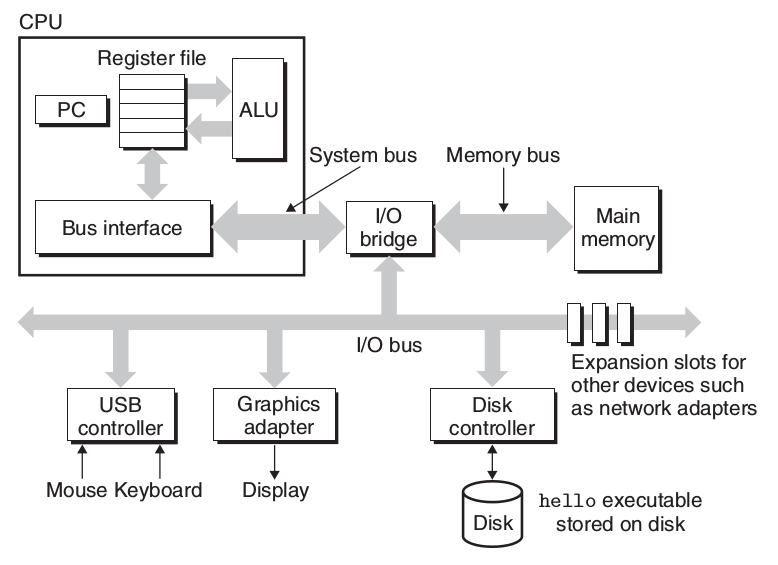
\includegraphics[keepaspectratio,width=0.3\paperwidth]{Pictures/sysBusCsapp.png}
		\caption{CSAPP:硬件体系结构}
	\label{fig:HardwareStructure}
	\end{center}
\end{figure}

\textbf{改进的哈佛结构},其结构特点为:
使用两个独立的存储器模块,分别存储指令和数据,每个存储模块都不允许指令和数据并存,以便实现并行处理;具有一条独立的地址总线和一条独立的数据总线,利用\textbf{公用地址总线}访问两个存储模块(程序存储模块和数据存储模块),\textbf{公用数据总线}则被用来完成程序存储模块或数据存储模块与CPU之间的数据传输;两条总线由程序存储器和数据存储器分时共用。

x86-64(简称x64)是64位版本的x86指令集,向前兼容于16位及32位的x86架构。x64于1999年由AMD设计,AMD首次公开64位集以扩充给x86,称为“AMD64”。其后也为英特尔所采用,现时英特尔称之为“Intel 64”,在之前曾使用过“Clackamas Technology” (CT)、“IA-32e”及“EM64T”。
Apple使用"x86-64"去称呼此64位架构。太阳微系统(已被甲骨文收购)及Microsoft称它为"x64"。BSD家族及其他Linux发布版则使用"amd64",32位版本则称为"i386"(或i486/586/686)。

\clearpage
%!Mode:: "TeX:UTF-8"
\section{多处理器架构}


从系统架构来看,目前的商用服务器大体可以分为三类,即对称多处理器结构(SMP:Symmetric Multi-Processor),非一致存储访问结构(NUMA:Non-Uniform Memory Access),以及海量并行处理结构(MPP:Massive Parallel Processing)。

\subsection{SMP(Symmetric Multi-Processor)}
所谓对称多处理器结构,是指服务器中多个CPU对称工作,无主次或从属关系。各CPU共享相同的物理内存,每个CPU访问内存中的任何地址所需时间是相同的,因此SMP也被称为一致存储器访问结构(UMA:Uniform Memory Access)。对SMP服务器进行扩展的方式包括增加内存、使用更快的CPU、增加CPU、扩充I/O(槽口数与总线数)以及添加更多的外部设备(通常是磁盘存储)。

SMP服务器的主要特征是共享,系统中所有资源(CPU、内存、I/O等)都是共享的。也正是由于这种特征,导致了SMP服务器的主要问题,那就是它的扩展能力非常有限。对于SMP服务器而言,每一个共享的环节都可能造成SMP服务器扩展时的瓶颈,而最受限制的则是内存。由于每个CPU必须通过相同的内存总线访问相同的内存资源,因此随着CPU数量的增加,内存访问冲突将迅速增加,最终会造成CPU资源的浪费,使CPU性能的有效性大大降低。实验证明,SMP服务器CPU利用率最好的情况是2至4个CPU。


\subsection{NUMA(Non-Uniform Memory Access)}

由于SMP在扩展能力上的限制,人们开始探究如何进行有效地扩展从而构建大型系统的技术,NUMA就是这种努力下的结果之一。
利用NUMA技术,可以把几十个CPU(甚至上百个CPU)组合在一个服务器内。

NUMA服务器的基本特征是具有多个CPU模块,每个CPU模块由多个CPU(如4个)组成,并且具有独立的本地内存、I/O槽口等。由于其节点之间可以通过互联模块(如称为Crossbar Switch)进行连接和信息交互,因此每个CPU可以访问整个系统的内存(这是NUMA系统与MPP系统的重要差别)。显然,访问本地内存的速度将远远高于访问远地内存(系统内其它节点的内存)的速度,这也是非一致存储访问NUMA的由来。由于这个特点,为了更好地发挥系统性能,开发应用程序时需要尽量减少不同CPU模块之间的信息交互。

利用NUMA技术,可以较好地解决原来SMP系统的扩展问题,在一个物理服务器内可以支持上百个CPU。比较典型的NUMA服务器的例子包括HP的Superdome、SUN15K、IBMp690等。
但NUMA技术同样有一定缺陷,由于访问远地内存的延时远远超过本地内存,因此当CPU数量增加时,系统性能无法线性增加。
如HP公司发布Superdome服务器时,曾公布了它与HP其它UNIX服务器的相对性能值,结果发现,64路CPU的Superdome (NUMA结构)的相对性能值是20,而8路N4000(共享的SMP结构)的相对性能值是6.3。从这个结果可以看到,8倍数量的CPU换来的只是3倍性能的提升。

\subsection{MPP(Massive Parallel Processing)}
和NUMA不同,MPP提供了另外一种进行系统扩展的方式,它由多个SMP服务器通过一定的节点互联网络进行连接,协同工作,完成相同的任务,从用户的角度来看是一个服务器系统。其基本特征是由多个SMP服务器(每个SMP服务器称节点)通过节点互联网络连接而成,每个节点只访问自己的本地资源(内存、存储等),是一种完全无共享(Share Nothing)结构,因而扩展能力最好,理论上其扩展无限制,目前的技术可实现512个节点互联,数千个CPU。目前业界对节点互联网络暂无标准,如NCR的Bynet,IBM的SPSwitch,它们都采用了不同的内部实现机制。但节点互联网仅供MPP服务器内部使用,对用户而言是透明的。

在MPP系统中,每个SMP节点也可以运行自己的操作系统、数据库等。但和NUMA不同的是,它不存在异地内存访问的问题。换言之,每个节点内的CPU不能访问另一个节点的内存。节点之间的信息交互是通过节点互联网络实现的,这个过程一般称为数据重分配(Data Redistribution)。

但是MPP服务器需要一种复杂的机制来调度和平衡各个节点的负载和并行处理过程。目前一些基于MPP技术的服务器往往通过系统级软件(如数据库)来屏蔽这种复杂性。举例来说,NCR的Teradata就是基于MPP技术的一个关系数据库软件,基于此数据库来开发应用时,不管后台服务器由多少个节点组成,开发人员所面对的都是同一个数据库系统,而不需要考虑如何调度其中某几个节点的负载。


\subsection{NUMA与MPP的区别}
从架构来看,NUMA与MPP具有许多相似之处:它们都由多个节点组成,每个节点都具有自己的CPU、内存、I/O,节点之间都可以通过节点互联机制进行信息交互。那么它们的区别在哪里?


首先是节点互联机制不同,NUMA的节点互联机制是在同一个物理服务器内部实现的,当某个CPU需要进行远地内存访问时,它必须等待,这也是NUMA服务器无法实现CPU增
加时性能线性扩展的主要原因。而MPP的节点互联机制是在不同的SMP服务器外部通过I/O 实现的,每个节点只访问本地内存和存储,节点之间的信息交互与节点本身的处理是并行进行的。因此MPP在增加节点时性能基本上可以实现线性扩展。

其次是内存访问机制不同。在NUMA服务器内部,任何一个CPU可以访问整个系统的内存,但远地访问的性能远远低于本地内存访问,因此在开发应用程序时应该尽量避免远地内存访问。在MPP服务器中,每个节点只访问本地内存,不存在远地内存访问的问题。


哪种服务器更加适应数据仓库环境?哪种服务器更加适应OLTP系统?
这需要从负载特征入手。众所周知,典型的数据仓库环境具有大量复杂的数据处理和综合分析,要求系统具有很高的I/O处理能力,并且存储系统需要提供足够的I/O带宽与之匹配。而一个典型的OLTP系统则以联机事务处理为主,每个交易所涉及的数据不多,要求系统具有很高的事务处理能力,能够在单位时间里处理尽量多的交易。显然这两种应用环境的负载特征完全不同。 

从NUMA架构来看,它可以在一个物理服务器内集成许多CPU,使系统具有较高的事务处理能力,由于远地内存访问时延远长于本地内存访问,因此需要尽量减少不同CPU模块之间的数据交互。显然,NUMA架构更适用于OLTP事务处理环境,当用于数据仓库环境时,由于大量复杂的数据处理必然导致大量的数据交互,将使CPU的利用率大大降低。

相对而言,MPP服务器架构的并行处理能力更优越,更适合于复杂的数据综合分析与处理环境。当然,它需要借助于支持MPP技术的关系数据库系统来屏蔽节点之间负载平衡与调度的复杂性。另外,这种并行处理能力也与节点互联网络有很大的关系。显然,适应于数据仓库环境的MPP服务器,其节点互联网络的I/O性能应该非常突出,才能充分发挥整个系统的性能。 










%!Mode:: "TeX:UTF-8"
\section{系统总线} 

\subsection{PCI}
外设互联标准(或称个人电脑接口,Personal Computer Interface),实际应用中简称为PCI(Peripheral Component Interconnect),是一种连接电子计算机主板和外部设备的总线标准。一般PCI设备可分为以下两种形式:
直接布放在主板上的集成电路,在 PCI 规范中称作“平面设备”(planar device);或者
安装在插槽上的扩展卡。
PCI bus常见于现代的个人计算机中,并已取代了ISA和VESA 局部总线,成为了标准扩展总线。PCI 总线亦常见于其他电子计算机类型中。PCI总线最终将被PCI Express和其他更先进的技术取代,这些技术现在已经被用于最新款的电子计算机中。
PCI 规范规定了该总线的物理尺寸(包括线宽)、电气特性、总线时序和协议。该规范可从美国PCI-SIG协会购得。
常见的PCI卡包括网卡、声卡、调制解调器、电视卡和磁盘控制器,还有USB和串口等端口。原本显卡通常也是PCI设备,但很快其带宽已不足以支持显卡的性能。PCI显卡现在仅用在需要额外的外接显示器或主板上没有AGP和PCI Express槽的情况。

\subsection{PCI-E}
PCI Express,简称PCI-E,是电脑总线PCI的一种,它沿用了现有的PCI编程概念及通讯标准,但建基于更快的串行通信系统。英特尔是该接口的主要支援者。PCIe仅应用于内部互连。由于PCIe是基于现有的PCI系统,只需修改物理层而无须修改软件就可将现有PCI系统转换为PCIe。PCIe拥有更快的速率,以取代几乎全部现有的内部总线(包括AGP和PCI)。英特尔希望将来能用一个PCIe控制器和所有外部设备交流,取代现有的南桥/北桥方案。

除了这些,PCIe设备能够支援热拔插以及热交换特性,支援的三种电压分别为+3.3V、3.3Vaux以及+12V。考虑到现在显卡功耗的日益增加,PCIe而后在规范中改善了直接从插槽中取电的功率限制,16x的最大提供功率达到了75W[1],比AGP 8X接口有了很大的提升。基本可以满足当时(2004年)中高阶显卡的需求。这一点可以从AGP、PCIe两个不同版本的6600GT显卡上就能明显地看到,后者并不需要外接电源。PCIe只是南桥的扩展总线,它与操作系统无关,所以也保证了它与原有PCI的兼容性,也就是说在很长一段时间内在主板上PCIe接口将和PCI接口共存,这也给用户的升级带来了方便。由此可见,PCIe最大的意义在于它的通用性,不仅可以让它用于南桥和其他设备的连接,也可以延伸到芯片组间的连接,甚至也可以用于连接图形芯片,这样,整个I/O系统重新统一起来,将更进一步简化计算机系统,增加计算机的可移植性和模块化。


\subsection{AGP}
AGP,全称为加速图像处理端口(Accelerated Graphics Port),是电脑主板上的一种高速点对点传输通道,供显卡使用,主要应用在三维电脑图形的加速上。AGP是在1997年由Intel提出,是从PCI标准上创建起来,是一种显卡专用接口。推出原因是为了消除PCI在处理3D图形时的瓶颈。AGP通常会被视为电脑总线的一种,但这样的分法严格来说是错误的;因为一组总线可容许多个设备共用,而AGP却不是。AGP不能多个插槽共用一组总线。一些主板设有多条独立的AGP插槽,现时AGP已基本被PCI Express所取代。


\subsection{LPC}
LPC总线,原名叫Low pin count Bus,是在IBM PC兼容机中用于把低带宽设备和“老旧”连接到CPU上。那些常见低速设备有:BIOS,串口,并口,PS/2的键盘和鼠标,软盘控制器,比较新的设备有可信平台模块。LPC总线通常和主板上的南桥物理相连,南桥在IBM PC AT平台上通常连接了一系列的“老旧”设备,例如两个可编程中断控制器, 可编程计时器和两个 ISA DMA 控制器。 LPC总线是Intel在1998时作为工业标准架构体系(ISA)的替代品引入,它与ISA在软件层面是类似的,尽管在物理层面是有着巨大不同的,ISA是16比特宽,8.33 MHz的总线,而它是4比特宽,有着四倍频率(33.3 MHz)的总线。 LPC总线最大的优点是只需要7个信号,在拥挤的现代主板上是很容易布局的。


\subsection{SPI}
SPI是很多术语的缩写。包括:
\subsubsection{serial peripheral interface}
序列周边接口(Serial Peripheral Interface Bus,SPI),类似I²C,是一种4线同步序列资料协定,适用于可携式装置平台系统,但使用率较I²C少。序列周边接口一般是4线,有时亦可为3线,有别于I²C的2线,以及1-Wire。

The Serial Peripheral Interface Bus or SPI (pronounced as either ess-pee-eye, spy or simply S.P.I) bus is a synchronous serial data link standard, named by Motorola, that operates in full duplex mode. Devices communicate in master/slave mode where the master device initiates the data frame. Multiple slave devices are allowed with individual slave select (chip select) lines. Sometimes SPI is called a four-wire serial bus, contrasting with three-, two-, and one-wire serial buses.
\subsubsection{System Packet Interface}
The System Packet Interface family of Interoperability Agreements from the Optical Internetworking Forum specify chip-to-chip, channelized, packet interfaces commonly used in synchronous optical networking and ethernet applications. A typical application of such a packet level interface is between a framer (for optical network) or a MAC (for IP network) and a network processor. Another application of this interface might be between a packet processor ASIC and a traffic manager device.

SPI-4.2 is a version of the System Packet Interface published by the Optical Internetworking Forum. It was designed to be used in systems that support OC-192 SONET interfaces and is sometimes used in 10 Gigabit Ethernet based systems.
SPI-4 is an interface for packet and cell transfer between a physical layer (PHY) device and a link layer device, for aggregate bandwidths of OC-192 Asynchronous Transfer Mode(ATM) and Packet over SONET/SDH (POS), as well as 10 Gigabit Ethernet applications.
A typical application of SPI-4.2 is to connect a framer device to a network processor. It has been widely adopted by the high speed networking marketplace.
The clocking is Source-synchronous and operates around 700 MHz. Implementations of SPI-4.2 have been produced which allow somewhat higher clock rates. This is important when overhead bytes are added to incoming packets.




\subsection{I2C}
I²C(Inter-Integrated Circuit)是内部整合电路的称呼,是一种串行通讯总线,使用多主从架构,由飞利浦公司在1980年代为了让主板、嵌入式系统或手机用以连接低速周边装置而发展。I²C的正确读法为``I-squared-C'' ,而``I-two-C''则是另一种错误但被广泛使用的读法,在中国则多以``I方C''称之。截至2006年11月1日为止,使用I²C协定不需要为其专利付费,但制造商仍然需要付费以获得I²C从属装置位址。


原始的I²C系统是在1980年代所建立的一种简单的内部总线系统,当时主要的用途在于控制由飞利浦所生产的芯片。
1992年完成了最初的标准版本释出,新增了传输速率为400 kbit/s的快速模式及长度为10位元的寻址模式可容纳最多1008个节点。1998年释出了2.0版,新增了传输速率为3.4Mbit/s的高速模式并为了节省能源而减少了电压及电流的需求。2.1版则在2001年完成,这是一个对2.0版做一些小修正,version 3.0, 2007年同时也是目前的最新版本。

在Linux中,I²C已经列入了核心模组的支援了,更进一步的说明可以参考核心相关的文件及位于/usr/include/linux/i2c.h 的这个标头档。OpenBSD则在最近的更新中加入了I²C的架构(framework)以支援一些常见的主控端控制器及感应器。

\subsection{UEXT}
Universal EXTension (UEXT) is a connector layout which includes power and three serials buses: Asynchronous, I2C, SPI. The connector layout was specified by Olimex Ltd and declared an open-project that is royalty-free.

\subsection{MII}
MII(Media Independent Interface,媒体独立接口),是与100Mbps的Ethernet PHY chip沟通时所使用的接口。

Being media independent means that different types of PHY devices for connecting to different media (i.e. Twisted pair copper, fiber optic, etc.) can be used without redesigning or replacing the MAC hardware. Thus any MAC may be used with any PHY, independent of the network signal transmission media.The MII can be used to connect a MAC to an external PHY using a pluggable connector, or direct to a PHY chip which is on the same printed circuit board.On a PC the CNR connector Type B carries MII bus interface signals.The MDIO Serial Management Interface (SMI) (see MDIO) is used to transfer management information between MAC and PHY.

Reduced Media Independent Interface (RMII) is a standard that addresses the connection of Ethernet physical layer transceivers (PHY) to Ethernet switches or the MAC portion of an end-device's Ethernet interface. It reduces the number of signals/pins required for connecting to the PHY from 16 (for an MII-compliant interface) to between 6 and 10. RMII is capable of supporting 10 and 100 Mbit/s; even 1 Gbit/s is possible, higher gigabit interfaces need a wider interface.

An Ethernet interface normally consists of 4 major parts: The MAC (Media Access Controller), the PHY (PHYsical Interface or transceiver), the magnetics, and the connector.

RMII is one of the possible interfaces between the MAC and PHY; others include MII and SNI, with additional wider interfaces (including XAUI, GBIC, SFP, SFF, XFP, and XFI) for gigabit and faster Ethernet links.

Gigabit Media Independent Interface (GMII) is an interface between the Media Access Control (MAC) device and the physical layer (PHY). The interface defines speeds up to 1000 Mbit/s.

RGMII uses half the number of data pins as used in the GMII interface. This reduction is achieved by clocking data on both the rising and falling edges of the clock in 1000 Mbit/s operation, and by eliminating non-essential signals.

The Serial Gigabit Media Independent Interface (SGMII) is a variant of MII, a standard interface used to connect an Ethernet MAC-block to a PHY. It is used for Gigabit Ethernet but can also carry 10/100 MBit Ethernet.

10 Gigabit Media Independent Interface (XGMII) is a standard defined in IEEE 802.3 for connecting full duplex 10 Gigabit Ethernet (10GbE) ports to each other and to other electronic devices on a printed circuit board.

XAUI是一个介于MAC到PHY之间电脑总线XGMII(10.0 Gbit/s)的延伸标准,XAUI发音``zowie'',与意味十倍的罗马数字 X 关联,是“附件单位接口”的起始。
XAUI是XGMII的延伸,XAUI位于MAC末端的XGXS、和PHY末端的XGXS之间。XAUI延伸了XGMII的操作长度并减少了信号接口的数目。应用范围包括延伸MAC和PHY模组之间的实体分隔以10.0 Gbit/s 以太系统分散横跨电路板。

The XGMII Extender, which is composed of an XGXS(The 10 Gigabit Ethernet Extended Sublayer) at the MAC end, an XGXS at the PHY end and a XAUI between them, is to extend the operational distance of the XGMII and to reduce the number of interface signals. Applications include extending the physical separation possible between MAC and PHY components in a 10 Gigabit Ethernet system distributed across a circuit board.


在10Mbps 以太网上,对应的是AUI, Attachment Unit Interface。

The MII design has been extended to support reduced signals and increases speeds. Current variants are Reduced Media Independent Interface, Gigabit Media Independent Interface, Reduced Gigabit Media Independent Interface, Serial Gigabit Media Independent Interface and 10 Gigabit Media Independent Interface.



























%!Mode:: "TeX:UTF-8"

\section{PC芯片组}
芯片组(chipset, PC chipset, or chip set)是一组共同工作的集成电路(“芯片”),并作为一个产品销售。它负责将电脑的核心——微处理器和机器的其他部分相连接,是决定主板级别的重要部件。以往,芯片组由多颗芯片组成,慢慢的简化为两颗芯片。

在计算机领域,“芯片组”术语通常是特指计算机主板或扩展卡上的芯片。当讨论基于英特尔的奔腾级处理器的个人电脑时,芯片组一词通常指两个主要的主板芯片组:北桥和南桥。芯片组的制造商可以,通常也是独立于主板的制造商。比如PC主板芯片组包括NVIDIA的nForce芯片组和威盛电子公司的KT880,都是为AMD处理器开发的,或英特尔许多芯片组。


\subsection{南北桥结构}

北桥(英语:Northbridge)是基于Intel处理器的个人电脑主板芯片组两枚芯片中的一枚,北桥设计用来处理高速信号,通常处理中央处理器、随机存取存储器、AGP或PCI Express的端口,还有与南桥之间的通信。


\tikzset{ box/.style={
rectangle, minimum width=1.3cm,very thick, draw=gray!50!black!50, text centered,
text width=0.2\textwidth, top color=white, bottom color=gray!50!black!20},
diamondbox/.style={diamond, 
draw=gray!50!black!, top color=white, bottom color=gray!50!black!10,
minimum width=3cm, minimum height=1.5cm, very thick, inner sep=0pt, text centered},
ellipbox/.style={ellipse,minimum width=1.3cm, minimum height=.8cm, draw=gray!50!black!, very thick, text width=0.07\textwidth, inner sep=0pt},
every node/.style={text badly centered, font=\footnotesize}
}

%自定义命令:用于流程图判断语句
\newcommand{\abovelabel}[1]{node[midway, above, text width=20mm]{#1}}
\newcommand{\rightlabel}[1]{node[midway, right]{#1}}


\begin{figure}[ht]
    \centering
    \begin{tikzpicture}
	\matrix[row sep=8mm, column sep=30mm]
	{
            &\node[box](cpu){CPU};&\node[box](cache){高速缓存};\\
            \node[box](graphic card){显卡槽};&\node[box](north){北桥};&\node[box](mem){内存};\\
            \node(usb){USB设备};&\node(south1){};&\node(ide){IDE硬盘};\\
            \node(isa){ISA设备(过时)};&\node(south2){};&\node(sata){SATA硬盘};\\
            \node(pci slots){PCI槽};&\node(south3){};&\node(onboard graph){Onboard显卡控制器};\\
            \node(phy){以太网};&\node(south4){};&\node(audio){声卡};\\
            \node(cmos){CMOS内存};&\node(south5){};&\node[box](flash rom){Flash Rom};\\
            &\node[box](super io){Super I/O};\\
	};

	\begin{scope}[every path/.style={draw, thick}]
            \path (cpu) -- (north) \rightlabel{FSB}; 
            \path (cpu) -- (cache) \abovelabel{BSB}; 
            \path (graphic card) -- (north) \abovelabel{高速图形总线(PCI-E或AGP)} -- (mem) \abovelabel{内存总线}; 
            \path (north) -- (south1) \rightlabel{桥间总线}; 
	    \path (usb) -- (south1) \abovelabel{USB总线}-- (ide) \abovelabel{IDE总线};
	    \path (isa) -- (south2) \abovelabel{ISA总线}-- (sata) \abovelabel{SATA总线};
	    \path (pci slots) -- (south3) \abovelabel{PCI总线}-- (onboard graph) \abovelabel{PCI总线};
	    \path (phy) -- (south4) \abovelabel{PCI等总线}-- (audio) \abovelabel{PCI总线};
	    \path (cmos) -- (south5) \abovelabel{PCI等总线} -- (flash rom) \abovelabel{LPC总线};
	    \path (south5) -- (super io) \rightlabel{LPC总线};
	\end{scope}
        
        \node[box, fit=(south1)(south5)](south){南桥};

    \end{tikzpicture}
    \caption{MainBoard}
\end{figure}

传统的北桥内建内存控制器,让处理器连接前端总线,而处理器和内存总线则跑相同的时脉。随后,芯片组分开处理器和内存总线的频率,让前端总线只代表处理器和北桥之间的通道。

北桥留下来的只剩下AGP或PCI Express控制器和与南桥通信,有时北桥会和南桥整合在同颗芯片中,有一些北桥则连绘图处理器也整合进去,而另外支援AGP或PCI Express接口。整合式北桥会侦测到附加在AGP插槽上有安装显卡,并停止其绘图处理器功能,但有些北桥可以允许同时使用整合式显卡和安装外加显卡,作为多显示输出。

南桥设计用来处理低速信号,通过北桥与CPU联系。各芯片组厂商的南桥名称都有所不同,例如英特尔称之为ICH,NVIDIA的称为MCP,ATI的称为IXP/SB。

南桥包含大多数周边设备接口、多媒体控制器和通讯接口功能。例如PCI控制器、ATA控制器、USB控制器、网络控制器、音效控制器。各世代的南桥效能大多雷同,但偶然听到某些南桥会有较差的Serial ATA或USB效能。目前所有的南桥制造商都提供SATA磁盘阵列功能,NVIDIA则允许SATA和ATA硬盘机混合组成磁盘阵列。最新的英特尔Matrix RAID技术,让RAID-0和RAID-1组态可以在两颗硬盘机中同时使用。

大多数南桥都能直接连接Gigabit Lan PHY(实体层芯片,用来处理连接讯号),高阶的南桥通常拥有两组Gigabit Lan PHY,不过中阶的主板则只支援一组。而NVIDIA最新的南桥则支援带宽合并、封包排序和TCP/IP加速等高级网络卡功能。现在大部份高级南桥则支援Azalia高传真音效,借着编码芯片支援7.1声道音效。

大多数南桥都支援PCI Express Hub,但主板制造商通常采用北桥所提供的PCI Express Lane。

存放BIOS配置信息的存储部件为CMOS内存,或称非易失性BIOS内存。传统上,BIOS信息存放于易失性的CMOS SRAM中,断点后借助电池的支持来保证信息不丢失。目前BIOS信息存放于EEPROM或flash中,电池只用于维持时钟硬件(RTC, real-time clocking)。CMOS RAM和电池都是南桥的一部分。

Super I/O可外接串口、并口(主要用于打印机)、PS/2鼠标和键盘、软盘、温度传感器和风扇转速监测等。Super I/O始于20世纪80年代,早期为附加芯片,后集成于主板。Super I/O早期用ISA总线同CPU通信。随着PCI总线的普及,Super I/O甚至成为主板上集成ISA总线的主要理由。后来Super I/O通过LPC(Low Pin Count)总线同CPU通信。Super I/O替主板实现了许多功能,简化主板设计,节约了成本。

Intel Hub Architecture(IHA)可用来取代南桥与北桥,IHA芯片组亦分成二大项:Graphics and Memory Controller Hub (GMCH)与I/O Controller Hub (ICH)。

随着Soc(System-on-a-Chip)技术的流行,现代设备逐渐将北桥集成到CPU冲模(die)上,而将南桥直接与CPU相连,如Intel的Sandy Bridge和AMD Fusion处理器(均发布于2011年)。预期于2013年发布的Intel Haswell将会把南桥与CPU集成到同一盒(package)中。

\subsection{单芯片芯片组}

AMD在Athlon 64时代将内存总线整个拿掉,直接设计到处理器中,让北桥的功能只是支援外加显卡接口,例如AGP和PCI Express x16。由于北桥的重要性降低,有厂商索性将南北桥合并,成为单一芯片组,例如NVIDIA的nForce 4。这样可以减低芯片组的制造成本,但电脑的效能会降低。

单芯片芯片组已推出多年,例如SiS 730。但直到最近nForce 4的出现才逐渐流行。现在的单芯片芯片组,不像以往般复杂,因Athlon 64已内建内存控制器,取代了北桥的功能。纵使芯片组变成单芯片,习惯上亦沿用旧名称。

\subsection{总线}

前端总线(FSB,Front Side Bus)是指中央处理器数据总线的专门术语,此总线负责中央处理器和北桥芯片间的数据传递。某些带有L2和L3缓存(Cache)的计算机,通过后端总线(Back Side Bus)实现这些缓存和中央处理器的连接,而此总线的数据传输速率总是高于前端总线。

大多数现代总线(GTL+和EV6)是CPU和芯片组的连接主干。芯片组(通常由南桥和北桥组成)是和系统中其他总线的连接节点。PCI、AGP和内存总线均和芯片组相连,以使设备间数据能相互传送。

这些第二级系统总线的运行速率取决于前端总线的速率。总之,高的前端总线速率意味着计算机的高处理性能。

早期连接南北桥的总线为PCI总线,现在主要是DMI(Intel)和UMI(AMD)。

在PC发展初期,由于处理器速度不高,大部份元件的时脉均保持同步,直至80486时代,在处理器制程持续进步下,处理器速度也加速成长,当时由于其他外部元件受电气结构所限,而无法跟进成长,因此Intel首次于处理器时脉中加入倍频设计,首颗处理器为Intel 80486DX2,外部传输时脉是处理器的一半,及后处理器成长速度仍远超过外部元件,两者速度差距越来越大。直至Pentium III时代,处理器时脉已超越1GHz,但外部传输时脉仍仅有133MHz。

正常来说,外频速度越高代表处理器在同一周期下可读写越多的数据,因此,外频速度很可能会变成系统效能上的瓶颈,为解决处理器带宽不足的问题,Intel于Pentium 4时代加入Quad Pumped Bus架构,使其在同一周期内可传送4笔数据,此举令外部传输时脉不变下,传输效率却可提升四倍。

前端总线(FSB、外频)的速度指的是CPU和北桥芯片间总线的速度。而系统总线(BusSpeed)的概念是建立在数位脉冲信号震荡速度基础之上的,也就是说,100MHz系统总线(BusSpeed)特指数位脉冲信号在每秒钟震荡一百万次,它更多的影响了PCI及其他总线的频率。之所以前端总线(FSB、外频)与系统总线(BusSpeed)这两个概念容易混淆,主要的原因是在以前的很长一段时间里,前端总线(FSB、外频)与系统总线(BusSpeed)是相同速率,因此往往直接称系统总线(BusSpeed)为外频,最终造成这样的误会。

中央处理器的时脉速度(简称内频)由系统总线速率(bus speed)乘上倍频系数决定。例如,一个时脉速度为 700MHz 的处理器,可能运行于 100MHz 的系统总线上。这说明处理器内的时钟倍频器的倍率设置为7,即中央处理器被设定为以7倍于系统总线的速率运行:100 MHz×7 = 700 MHz。通过改变倍频系数或系统总线速率,可以得到不同的时脉速度。















%!Mode:: "TeX:UTF-8"
 
\section{缓存}
\cite{wikipedia}:

\subsection{CPU高速缓存结构}
m位地址,有$m=t+s+b$, 寻址空间$M=2^m$, 缓存容量$C=S \times E \times B=2^s E 2^b$, $C<M$则$E < 2^t$.

直接相连:$E=1$.
全相连:$S=1$.


\begin{figure}[ht]
	\begin{center}
	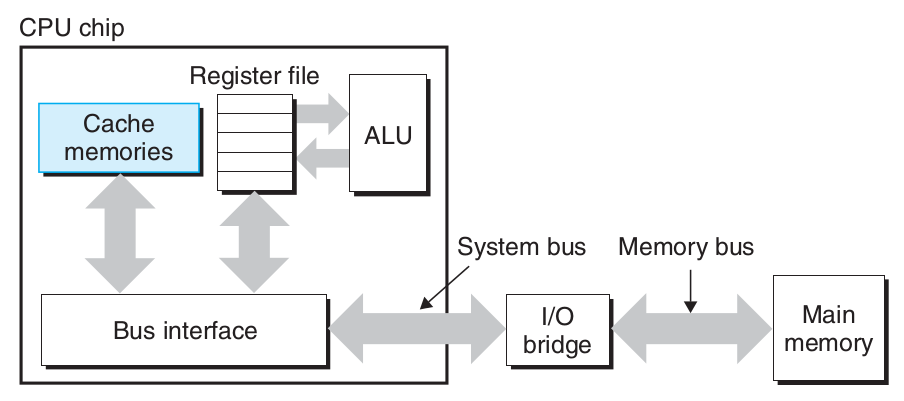
\includegraphics[keepaspectratio,width=0.3\paperwidth]{Pictures/cacheBus.png}
		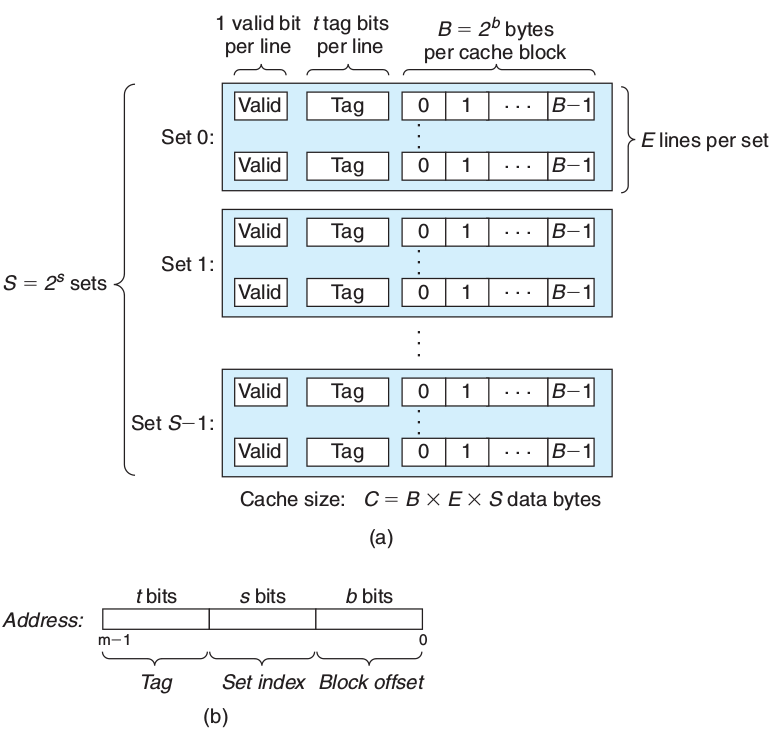
\includegraphics[keepaspectratio,width=0.3\paperwidth]{Pictures/cache.png}
	\caption{高速缓存通用结构}
	\label{fig:cacheMemStructure}
	\end{center}
\end{figure}


\subsection{TLB}
分页表是一种数据结构,用于计算机操作系统中的虚拟内存系统,存储了虚拟地址到物理地址间的映射。虚拟地址在访问进程中是唯一的,物理地址在硬件中是唯一的。比如RAM。CPU的内存管理单元(memory management unit MMU)存储最近用过的映射缓存,来自操作系统分页表。被称为转译后备缓冲器(translation lookaside buffer, TLB)。TLB是一个索引缓存。

转译后备缓冲器(英文:Translation Lookaside Buffer,首字母缩略字:TLB),在中国大陆也被翻译为页表缓存、转址旁路缓存,为CPU的一种缓存,由存储器管理单元用于改进虚拟地址到物理地址的转译速度。目前所有的桌面型及服务器型处理器(如 x86)皆使用TLB。TLB具有固定数目的空间槽,用于存放将虚拟地址映射至物理地址的标签页表条目。为典型的内容可寻址存储器(content-addressable memory,首字母缩略字:CAM)。其搜索关键字为虚拟内存地址,其搜索结果为物理地址。如果请求的虚拟地址在TLB中存在,CAM 将给出一个非常快速的匹配结果,之后就可以使用得到的物理地址访问存储器。如果请求的虚拟地址不在 TLB 中,就会使用标签页表进行虚实地址转换,而标签页表的访问速度比TLB慢很多。有些系统允许标签页表被交换到次级存储器,那么虚实地址转换可能要花非常长的时间。

在任务(task)切换时,部分 TLB 条目可能会失效,例如先前运行的进程已访问过一个页面,但是将要执行的进程尚未访问此页面。最简单的策略是清出整个 TLB。

多核系统的每个核都有自己的TLB。与cache不同,TLB不需要核间同步,因为每个核运行的进程有不同的地址映射。


\subsection{缓存一致性}
分布式共享内存(Distributed Shared Memory,DSM)指物理上分布式的内存可以在逻辑上被当做一块内存来访问。这里的共享指的是地址空间的共享。
为维护“内存一致性”(memory coherence),需选择一个“一致性协议”(coherence protocol)来实现一种"一致性模型"(consistency model)。
DSM系统的实例包括OpenSSI,MOSIX,Kerrighed,TreadMarks等。注意同“分布式缓存”区分开。

\begin{quotation}
分布式缓存(Distributed cache)是对传统意义上单点缓存概念的扩展,使得缓存可以跨越多个服务器。
由于主存变得便宜,以及网卡速度的增强,分布式缓存得以变得现实。
分布式缓存的例子包括:Oracle Coherence, Ehcache, Hazelcast, Memcached, SafePeak, Riak, Redis等。
\end{quotation}

在多核系统下也存在内存一致性问题。
如果多核同时访问同一共享内存区,且存在写操作,就可能出现缓存一致性(内存一致性)问题,即某核读到的本地缓存副本不是最新的。
需要引入“内存一致性协议”(memory coherence protocol)来解决这个问题。

一致性的实现方式包括:
\begin{description}
\item[基于目录的实现(Directory-based)]目录维护各缓存间的一致性信息。处理器在将内存值加载到本地cache时时必须先查询目录。
当某一表项被更新时,目录要么标记其失效,要么主动更新所有其他缓存。
\item[Snooping]每一个本地cache监控地址线,如果一个内存更新访问涉及自己所缓存的对象,那么本地缓存的这个副本应被失效。
\end{description}
这些实现机制可用于多核、多处理器缓存,以及分布式共享内存系统。

一致性模型"(consistency model)包括:
\begin{description}
\item[线性一致性(Linearizability)]或严格一致性(Strict consistancy)、原子一致性(Atomic consistancy):任何对一个内存位置X的读操作,将返回最近一次对该内存位置的写操作所写入的值。
\item[顺序一致性(sequential consistency)](并发程序在多处理器上的)任何一次执行结果都相同,就像所有处理器的操作按照某个顺序执行,各个微处理器的操作按照其程序指定的顺序进行。
换句话说,所有的处理器以相同的顺序看到所有的修改。读操作未必能及时得到此前其他处理器对同一数据的写更新。但是各处理器读到的该数据的不同值的顺序是一致的。
\item[释放一致性(Release consistency )]
同步操作被分裂成获得(acquire)和释放(release)操作。
如果某进程的写操作在该进程执行释放之后、在其他进程执行获取之前被看到,则称释放一致性。
释放一致性可以通过两种一致性协议来实现:
一致性操作(coherence actions)可以在退出临界区时完成(渴望释放一致性),也可推迟到下一次进入临界区(懒惰释放一致性)。
\item[因果一致性(Causal consistency )]
因果一致的存储器应遵守以下条件:可能因果相关的写操作应对所有进程可见,且顺序一致。并发写操作在不同机器看来顺序可能是不同的。
如果进程A通知进程B它已更新了一个数据项,那么进程B的后续访问将返回更新后的值,且一次写入将保证取代前一次写入。与进程A无因果关系的进程C的访问遵守一般的最终一致性规则。因果一致性弱于顺序一致性,强于PRAM一致性。
假设进程P1写变量x,然后P2读出x,写入y。这里读出x和写入y之间可能有潜在的因果联系,因为y的计算很可能决定于P2读到的x值(即P1写入的值)。 另一方面,若两进程自然而同时地写两个变量,就没有因果联系。先有读操作之后执行写操作,两个事件就可能有因果联系。相似的,读和提供所读数据的写有因果关系。没有因果关系的操作称为并发的(concurrent)。
\item[PRAM(Piplined RAM)一致性]又称FIFO一致性,几乎等同于处理机一致性(Processor consistency)。
一个进程(处理机)的多个写操作被另一进程按照相同的顺序接收到,如同在流水线中到达一样,但来自多个进程的写操作顺序不定。PRAM一致性很容易实现。
对于双处理器,处理器一致性与顺序一致性是等价的。
\item[Delta一致性]在固定时间Delta之内达到全局一致。
\item[弱一致性]弱一致性有三个属性:a. 对同步变量的访问是顺序一致的;
b. 在所有先前的写操作完成之前,不能访问同步变量;
c. 在先前所有同步变量的访问完成前,不能访问(读或写)数据。
\end{description}













\clearpage
%!Mode:: "TeX:UTF-8"
\section{磁盘控制器技术}


\subsection{IDE与ATA}
IDE(Integrated Drive Electronics)是一种计算机系统接口,主要用于硬盘和CD-ROM,
本意为“把控制器与盘体集成在一起的硬盘”,
与ATA(Advanced Technology Attachment)关系密切。
数年以前PC主机使用的硬盘,大多数都是IDE兼容的,只需用一根电缆将它们与主板或适配器连起来就可以了,而目前主要接口为SATA接口。
一般说来,ATA是一个控制器技术,而IDE是一个匹配它的磁盘驱动器技术,但是两个术语经常可以互用。
ATA是一个花费低而性能适中的接口,主要是针对台式机而设计的,销售的大多数ATA控制器和IDE磁盘都是更高版本的,
称为ATA - 2和ATA - 3,与之匹配的磁盘驱动器称为增强的IDE。


把盘体与控制器集成在一起的做法,减少了硬盘接口的电缆数目与长度,数据传输的可靠性得到了增强,硬盘制造起来变得更容易,
因为厂商不需要再担心自己的硬盘是否与其他厂商生产的控制器兼容,对用户而言,硬盘安装起来也更为方便。
ATA是用传统的40-pin并行数据线连接主板与硬盘的,外部接口速度最大为133MB/s,因为并行线的抗干扰性太差,且排线占空间,不利散热,而逐渐被SATA所取代。
ATA主机控制器芯片差不多集成到每一个生产的系统板,提供连接4个设备的能力。
ATA控制器已经变得非常廉价和常见,但在SATA技术日益发展下,没有ATA的主版已经出现,
而且Intel在新型的芯片组中已经不默认支持ATA接口,主机版厂商需要另加芯片去对ATA作出支持(通常是为了兼容旧有硬盘和光盘驱动器)。

普遍情况下,一块主板只有两个IDE接口,每个接口可以挂两个IDE设备。
但同一个接口的两个设备是共用带宽的,对速度的影响非常大。所以稍有常识的人,都会把硬盘和光驱分开两条IDE线连接到主板上 
这样,IDE有个很大的问题,就是虽然一块主板可以连接4个设备,但事实上只要超过两个,速度就大大下降。
更大的问题是,同一条线上两个设备要严格按主/从设置才能正常运行。

并行ATA在支持设备热插拔方面能力有限,这一点对服务器方面的应用非常重要。因为服务器通常采用RAID的方式,
任何一块硬盘坏了都可以热拔插更换,而不影响数据的完整性,确保服务器任何情况下都正常开着。
具有热插拔支持功能的SCSI和光纤通道占据了企业级应用的几乎全部市场,
并行ATA空有价格优势而不能获得一席之地,主要原因就是它不支持热拔插。 


\subsection{SCSI}
小型计算机系统接口(SCSI,Small Computer System Interface)是一种用于计算机及其周边设备之间(硬盘、软驱、光驱、打印机、扫描仪等)系统级接口的独立处理器标准。
SCSI标准定义了命令、通信协定以及实体的电气特性(换成OSI的说法,就是占据了实体层、链接层、通信层、应用层),
最大部份的应用是在存储设备上(例如硬盘、磁带机),但SCSI可以连接的设备也包括扫描仪、光学设备(像CD、DVD)、打印机等等,

系统中的每个SCSI设备都必须有自己唯一的ID(标识号),在8-bit总线上,这个号码是0~7;在16-bit总线上,这个号码从0~15。
SCSI Adapter系统默认ID为7。
SCSI链的最后一个SCSI设备要用终结器,中间设备是不需要终结器的。
一旦中间设备使用了终结器,那么SCSI卡就无法找到以后的SCSI设备了。

SCSI-1是最初版本的SCSI,现已过时。
SCSI-1具有8位BUS,数据传输率为40 Mbps(5 MB/sec)。
SCSI-2是基于CCS的SCSI-1改进版本。
在Fast SCSI和Wide SCSI的支持下,SCSI-2在原SCSI-1的基础上传输速率得到了提高。
Fast SCSI的传输速率为10 MB/sec,当配合16位BUS时,其传输速率为20 MB/sec(Fast-Wide SCSI)。
当今,SCSI-3单元采用Ultra-Wide和Ultra SCSI类型的驱动器。
Ultra SCSI具有8位BUS,其传输速率为20 MB/sec。
Ultra-Wide SCSI具有16位BUS,其传输速率达到40 MB/sec。 
SCSI-3在SCSI-2基础上有了很多提高,如串行SCSI。通过6芯同轴电缆,其传输速率达到100 MB/sec。
SCSI-3解决了旧SCSI版本中存在的终结和延迟问题,
此外通过即插即用(plug-and-play)操作,自动分配SCSI ID和终结,使SCSI安装更为容易。
与SCSI-2支持8台设备相比,SCSI-3能支持32台设备。

同SCSI相比,IDE还具有性能价格比高、适用面广等特点。
个人电脑用户不但需要配置的外设不多,而且对速度要求也不高,因此选用IDE接口比SCSI更合适些。
SCSI相比于IDE的优势包括:
1)
IDE的工作方式需要CPU的全程参与,CPU读写数据的时候不能再进行其他操作,
而SCSI接口,则完全通过独立的高速的SCSI卡来控制数据的读写操作。
IDE接口为改善这个问题也做了很大改进,已经可以使用DMA模式而非PIO模式来读写,
对CPU的占用可大大减小。尽管如此,比较SCSI和IDE在CPU的占用率,还是可以发现SCSI仍具有相当的优势。
2)SCSI的扩充性比IDE大,一般每个IDE系统可有2个IDE通道,总共连4个IDE设备,而SCSI接口可连接7—15个设备,比IDE要多很多,而且连接的电缆也远长于IDE。
3)虽然SCSI设备价格高些,与IDE相比,SCSI的性能更稳定、耐用,可靠性也更好。
4)SCSI还允许在对一个设备传输数据的同时,另一个设备对其进行数据查找。
这就可以在多任务操作系统如Linux、WindowsNT中获得更高的性能。


\subsection{SATA}
Serial ATA(SATA, 串行ATA,Serial Advanced Technology Attachment),
是串行SCSI(SAS:Serial Attached SCSI)的孪生兄弟,两者的排线兼容,SATA硬盘可接上SAS接口。
它是一种电脑总线,主要功能是用作主板和大量存储设备(如硬盘及光盘驱动器)之间的数据传输之用。

在数据传输上这一方面,SATA的速度比以往更加快捷,并支持热插拔。
另一方面,SATA总线使用了嵌入式时钟频率信号,具备了比以往更强的纠错能力,能对传输指令(不仅是数据)进行检查,提高了数据传输的可靠性。
不过,SATA和以往最明显的分别,是用上了较细的排线,有利机箱内部的空气流通,某程度上增加了整个平台的稳定性。
SATA与原来的IDE相比有很多优越性,最明显的就是数据线从80 pin变成了7 pin,
而且IDE线的长度不能超过0.4米,而SATA线可以长达1米,安装更方便,利于机箱散热。
每个设备都直接与主板相连,独享150M字节/秒带宽,设备间的速度不会互相影响。
热拔插对于普通家庭用户来说可能作用不大,但对于服务器却是至关重要。
事实上,SATA在低端服务器应用上取得的成功,远比在普通家庭应用中的影响力大。
SATA提高了错误检查的能力,除了对CRC对数据检错之外,还会对命令和状态包进行检错,
因此和并行ATA相比提高了接入的整体精确度,使串行ATA在企业RAID和外部存储应用中具有更大的吸引力。 


现时,SATA分别有SATA 1.5Gbit/s、SATA 3Gbit/s和SATA 6Gbit/s三种规格。
SATA 1.5Gb/s为第一代SATA接口,坊间的非官方名称为SATA-1。
SATA 3Gb/s在2004年正式推出,坊间的非官方名称为SATA-2(SATA-II),符合ATA-7规范,传输速度可达3.0Gbit/s。
在SATA2.0扩展规范所带来的一系列新功能中,NCQ(Native Command Queuing,原生命令队列)功能最令人关注。
SATA 6Gb/s 在2009年5月26日SATA-IO 完成 SATA 3.0 最终规格发布,比上一代提升一倍速率至6Gb/s,
此外增加多项新技术,包涵新增 NCQ 指令以改良传输技术,并减低传输时所需耗电量。
SATA不依赖于系统总线的带宽,而是内置时钟,每一代SATA升级带宽的增加都是成倍的,这点和PATA的一级级算术级数增长是不同的。
所谓3Gb/s的算法,3000MHz的频率 x 每次发送一个数据 x 80\%(8b/10b的编码) / 8 bits per byte = 300Mbytes/s,
同理1.5Gb/s也是这样可算成150MB/s,
也就是一般我们在买硬盘时,有时候会看到SATA 150MB/s / 300MB/s,有时候又会看到SATA 1.5Gb/s / 3Gb/s的缘故。
以USB 3.0而言,它拥有5Gbps的带宽,折算为500Mbytes/s,所以USB 3.0的带宽比SATA 3.0的600MB/s还来的小。

SATA的诸多先进性总体上对个人电脑用户意义不是太大,
它最大的意义的反而是适应了入门级企业应用的需要。 
但在企业级应用方面,它又仍然在很多方面有待改进:
单线程的机械底盘(不适应服务器应用程序大量非线性的读取请求。所以SATA硬盘用来做视频下载服务器还不错,用在网上交易平台则力不从心),
形同虚设的热拔插功能(SATA硬盘虽然可以热拔插,但SATA组成的阵列在某块硬盘损坏的时候,不能象SCSI、FC和SAS那样,具有SAF-TE机制用指示灯显示,知道具体坏的是哪一块)。
SATA 1.0控制器的传输速度效率不高,虽然标称具有150MB/s的峰值速度,事实上最快的SATA硬盘速度也只有60MB/s。
虽然SATA硬盘相对于SCSI硬盘来说很便宜,但整个的SATA方案并不便宜。
主要原因是SATA 1.0控制器的每个接口只能连接一个硬盘,8个硬盘组成的阵列需要8个接口,把每个接口300多元的花费算进去,就不便宜了。 

SATA国际组织(Serial ATA International Organization)正在着手制定下一代SATA标准,
定名为SATA Express,带宽最高可达8Gbps和16Gbps。 要达到最高的16Gbps带宽(现在最快的SATA 3.0标准带宽为6Gbps),
SATA Express标准将会如其名称所描述的,把SATA软件架构和PCI-Express高速界面结合在一起。
SATA国际组织称SATA Express标准将会带来新一代更快的存储装置和对应的主板接口,并且还能兼容现有的SATA设备。 S
ATA国际组织主席Mladen Luksic称该标准将使固态与混合硬盘受益于新一代PCI-Express 3.0的高带宽从而打破性能瓶颈,
标准的具体细节将在年内制定完成。 
SATA国际组织同时表示除SATA Express外,还有针对集成在主板上的嵌入式单芯片SSD存储解决方案的SATA µSSD标准,面向移动设备如平板电脑等。
SATA Express还处于标准制定阶段,可能会是SATA 3.2规范的一部分。
它其实就是PCI-E物理层上的SATA链接层,同时保持了对SATA 3/6Gbps等旧版规范的兼容(当然性能也会受影响),
传输带宽最初预计的范围是8-16Gbps,基本已经确定会达到10Gbps,实际传输速度也有1GB/s,比SATA 6Gbps要快将近70%。





\subsection{SAS}

SAS(Serial Attached SCSI)是并行SCSI接口之后开发出的全新接口。
此接口的设计是为了改善存储系统的效能、可用性和扩充性,
提供与串行ATA (Serial ATA,缩写为SATA)硬盘的兼容性。

SAS的接口技术可以向下兼容SATA。
SAS系统的背板(Backpanel)既可以连接具有双端口、高性能的SAS驱动器,也可以连接高容量、低成本的SATA驱动器。
因为SAS驱动器的端口与SATA驱动器的端口形状看上去类似,所以SAS驱动器和SATA驱动器可以同时存在于一个存储系统之中。
但需要注意的是,SATA系统并不兼容SAS,所以SAS驱动器不能连接到SATA背板上。
由于SAS系统的兼容性,IT人员能够运用不同接口的硬盘来满足各类应用在容量上或效能上的需求,
因此在扩充存储系统时拥有更多的弹性,让存储设备发挥最大的投资效益。


第一代SAS为数组中的每个驱动器提供 3.0 Gbps(300 MB/s)的传输速率(现在主流Ultra 320 SCSI速度为320MB/s)。
第二代SAS为数组中的每个驱动器提供 6.0 Gbps(600 MB/s)的传输速率。

SAS由3种类型协议组成,根据连接的不同设备使用相应的协议进行数据传输:
串行SCSI协议 (SSP) — 用于传输SCSI命令。
SATA通道协议 (STP) — 用于传输SATA数据。
SCSI管理协议 (SMP) — 用于对SAS设备的维护和管理。

SAS的接口技术可以向下兼容SATA。
具体来说,二者的兼容性主要体现在物理层和协议层的兼容。
在物理层,SAS接口和SATA接口完全兼容,SATA硬盘可以直接使用在SAS的环境中,
从接口标准上而言,SATA是SAS的一个子标准,因此SAS控制器可以直接操控SATA硬盘,
但是SAS却不能直接使用在SATA的环境中,因为SATA控制器并不能对SAS硬盘进行控制;
在协议层,SAS由3种类型协议组成,根据连接的不同设备使用相应的协议进行数据传输。其中串行SCSI协议(SSP)用于传输SCSI命令;SCSI管理协议(SMP)用于对连接设备的维护和管理;
SATA通道协议(STP)用于SAS和SATA之间数据的传输。
因此在这3种协议的配合下,SAS可以和SATA以及部分SCSI设备无缝结合。

存储设备的反应速度,除了各环节间的配合与操作系统的影响之外,硬盘的反应速度其实具有关键性的地位。
企业级的工作站或存储设备,一般来说,都采用光纤信道(Fibre Channel,FC)与SCSI硬盘作为内部的存储媒体。
但是随着SCSI硬盘在扩增性上的限制,SAS(Serial Attached SCSI)硬盘崭露头角。
服务器厂商有越来越多采用SAS硬盘作为内部的存储媒体,小型负载的应用可以采用SAS硬盘,可兼具预算与效能的考虑。


SAS目前的不足主要有以下方面:
1)硬盘、控制芯片种类少:只有希捷、迈拓以及富士通等为数不多的硬盘厂商推出了SAS接口硬盘.
2)硬盘价格太贵:比起同容量的Ultra 320 SCSI硬盘,SAS硬盘要贵了一倍还多。
3)实际传输速度变化不大:SAS硬盘的接口速度并不代表数据传输速度,受到硬盘机械结构限制,现在SAS硬盘的机械结构和SCSI硬盘几乎一样。
目前数据传输的瓶颈集中在由硬盘内部机械机构和硬盘存储技术、磁盘转速所决定的硬盘内部数据传输速度,也就是80MBsec左右,SAS硬盘的性能提升不明显。
4)用户追求成熟、稳定的产品. 虽然SAS接口服务器和SCSI接口产品在速度、稳定性上差不多,但目前的技术和产品都还不够成熟。
不过随着英特尔等主板芯片组制造商、希捷等硬盘制造商以及众多的服务器制造商的大力推动,SAS的相关产品技术会逐步成熟,价格也会逐步滑落,早晚都会成为服务器硬盘的主流接口。

衡量一种技术的优劣通常有4个基本指标,即性能、可靠性、可扩展性和成本。
回顾串行磁盘技术的发展历史,从光纤通道,到SATA,再到SAS,几种技术各有所长。
光纤通道最早出现的串行化存储技术,可以满足高性能、高可靠和高扩展性的存储需要,但是价格居高不下;
SATA硬盘成本倒是降下来了,但主要是用于近线存储和非关键性应用,毕竟在性能等方面差强人意;
SAS应该算是个全才,可以支持SAS和SATA磁盘,很方便地满足不同性价比的存储需求,是具有高性能、高可靠和高扩展性的解决方案。











%!Mode:: "TeX:UTF-8"
\section{嵌入式多核处理器}
多核处理器目前发展非常迅速,主流厂商主要包括CAVIUM的OCTEON系列,RMI的XLR系列,飞思卡尔的PPC QorIQ系列.其中CAVIUM在业界处于领先定位,RMI在国内市场具有优势,而飞思卡尔由于研发速度较慢,其全新的多核处理器一直没有正式上市.目前国内华为,中兴等通信厂商,已经或者正在准备,把原有的通信产品移植到多核处理器上开发,以便降低成本和提高性能.



%!Mode:: "TeX:UTF-8"
\section{RAID阵列}

独立硬盘冗余阵列(RAID, Redundant Array of Independent Disks),其基本思想就是把多个相对便宜的硬盘组合起来,成为一个硬盘阵列组,使性能达到甚至超过一个价格昂贵、容量巨大的硬盘。根据选择的版本不同,RAID比单颗硬盘有以下一个或多个方面的好处:增强数据集成度,增强容错功能,增加处理量或容量。

\begin{figure}[ht]
	\begin{center}
		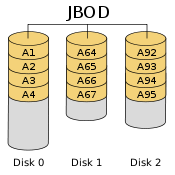
\includegraphics[keepaspectratio,width=0.15\paperwidth]{Pictures/RAID/JBOD.png}
		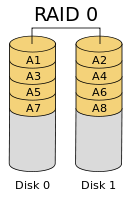
\includegraphics[keepaspectratio,width=0.1\paperwidth]{Pictures/RAID/RAID0.png}
		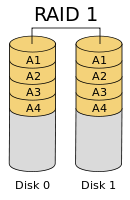
\includegraphics[keepaspectratio,width=0.1\paperwidth]{Pictures/RAID/RAID1.png}
	\end{center}
\end{figure}

\textbf{RAID 0}亦称为带区集。它将两个以上的磁盘串联起来,成为一个大容量的磁盘。在存放数据时,分段后分散存储在这些磁盘中,因为读写时都可以并行处理,所以在所有的级别中,RAID 0的速度是最快的。但是RAID 0既没有冗余功能,也不具备容错能力,如果一个磁盘(物理)损坏,所有数据都会丢失,危险程度与\textbf{JBOD}相当。


\begin{figure}[ht]
	\begin{center}
		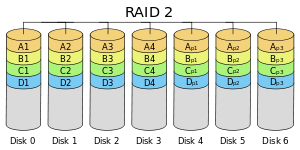
\includegraphics[keepaspectratio,width=0.2\paperwidth]{Pictures/RAID/RAID2.png}
		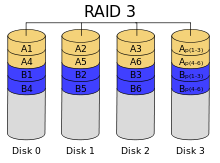
\includegraphics[keepaspectratio,width=0.2\paperwidth]{Pictures/RAID/RAID3.png}
	\end{center}
\end{figure}

两组以上的N个磁盘相互作镜像,在一些多线程操作系统中能有很好的读取速度,理论上读取速度等于硬盘数量的倍数,另外写入速度有微小的降低。只要一个磁盘正常即可维持运作,可靠性最高。\textbf{RAID 1}就是镜像,其原理为在主硬盘上存放数据的同时也在镜像硬盘上写一样的数据。当主硬盘(物理)损坏时,镜像硬盘则代替主硬盘的工作。因为有镜像硬盘做数据备份,所以RAID 1的数据安全性在所有的RAID级别上来说是最好的。但无论用多少磁盘做RAID 1,仅算一个磁盘的容量,是所有RAID中磁盘利用率最低的一个级别。

\begin{figure}[ht]
	\begin{center}
		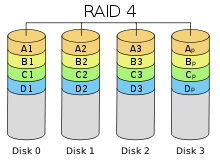
\includegraphics[keepaspectratio,width=0.2\paperwidth]{Pictures/RAID/RAID4.png}
		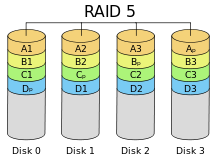
\includegraphics[keepaspectratio,width=0.2\paperwidth]{Pictures/RAID/RAID5.png}
		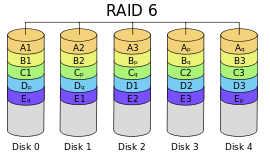
\includegraphics[keepaspectratio,width=0.2\paperwidth]{Pictures/RAID/RAID6.png}
	\end{center}
\end{figure}

\textbf{RAID 2}是RAID 0的改良版,以汉明码的方式将数据进行编码后分区为\textbf{独立的比特},并将数据分别写入硬盘中。因为在数据中加入了错误修正码(ECC,Error Correction Code),所以数据整体的容量会比原始数据大一些,RAID2最少要三台磁盘驱动器方能运作。RAID 2技术实施复杂,在商业环境中很少使用,早已被淘汰。

\begin{figure}[ht]
	\begin{center}
		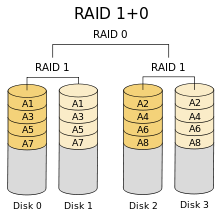
\includegraphics[keepaspectratio,width=0.2\paperwidth]{Pictures/RAID/RAID10.png}
		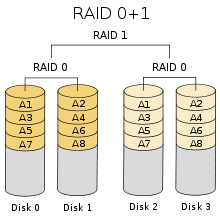
\includegraphics[keepaspectratio,width=0.2\paperwidth]{Pictures/RAID/RAID01.png}
	\end{center}
\end{figure}
\textbf{RAID 3}同RAID 2非常类似,都是将数据条块化分布于不同的硬盘上,区别在于RAID 3使用简单的奇偶校验,并用单块磁盘存放奇偶校验信息。如果一块磁盘失效,奇偶盘及其他数据盘可以重新产生数据;如果奇偶盘失效则不影响数据使用。


\textbf{RAID 4}与RAID 3不同的是它在分区时是以区块为单位分别存在硬盘中(块交织技术,Block interleaving),但每次的数据访问都必须从同比特检查的那个硬盘中取出对应的同比特数据进行核对,由于过于频繁的使用,所以对硬盘的损耗可能会提高。RAID 4使用一块磁盘作为奇偶校验盘,每次写操作都需要访问奇偶盘,这时奇偶校验盘会成为写操作的瓶颈。RAID 4在商业环境中也很少使用,面临淘汰。



\textbf{RAID 5是一种储存性能、数据安全和存储成本兼顾的存储解决方案}。它使用的是Disk Striping(硬盘分区)技术。RAID 5至少需要三颗硬盘,RAID 5不是对存储的数据进行备份,而是把数据和相对应的奇偶校验信息存储到组成RAID5的各个磁盘上,并且奇偶校验信息和相对应的数据分别存储于不同的磁盘上。当RAID5的一个磁盘数据发生损坏后,可以利用剩下的数据和相应的奇偶校验信息去恢复被损坏的数据。RAID 5可以理解为是RAID 0和RAID 1的折衷方案。RAID 5可以为系统提供数据安全保障,但保障程度要比镜像低而磁盘空间利用率要比镜像高。RAID 5具有和RAID 0相近似的数据读取速度,只是因为多了一个奇偶校验信息,写入数据的速度相对单独写入一块硬盘的速度略慢,若使用“回写高速缓存”可以让性能改善不少。同时由于多个数据对应一个奇偶校验信息,RAID 5的磁盘空间利用率要比RAID 1高,存储成本相对较便宜。


与RAID 5相比,RAID 6增加了第二个独立的奇偶校验信息块。两个独立的奇偶系统使用不同的算法,数据的可靠性非常高,即使两块磁盘同时失效也不会影响数据的使用。但RAID 6需要分配给奇偶校验信息更大的磁盘空间,相对于RAID 5有更大的“写损失”,因此“写性能”非常差。较差的性能和复杂的实作方式使得\textbf{RAID 6很少得到实际应用}。同一数组中最多容许两个磁盘损坏。更换新磁盘后,数据将会重新算出并写入新的磁盘中。依照设计理论,RAID 6必须具备四个以上的磁盘才能生效。


RAID 10是先镜射再分区数据,再将所有硬盘分为两组,视为是RAID 0的最低组合,然后将这两组各自视为RAID 1运作。

RAID 01则是跟RAID 10的程序相反,是先分区再将数据镜射到两组硬盘。它将所有的硬盘分为两组,变成RAID 1的最低组合,而将两组硬盘各自视为RAID 0运作。当RAID 10有一个硬盘受损,其余硬盘会继续运作。RAID 01只要有一个硬盘受损,同组RAID 0的所有硬盘都会停止运作,只剩下其他组的硬盘运作,可靠性较低。因此,\textbf{RAID 10远较RAID 01常用}。



\clearpage



%!Mode:: "TeX:UTF-8"
\section{Rack-Mountable Equipment}

A \textbf{rack} is the whole cabinet that is usually 42-U tall.

A \textbf{rack rail} is a verticall-stretching metal slice on each side of a
server rack with wholes for fastening.

A \textbf{chassis} might refer to a support board on top of each shelf.

1U, 1 RACK UNIT,=1.752 inches (44.50 mm)


\bibliographystyle{unsrt}
\bibliography{thebib}



\end{document}
